\chapter{Guest Speaker Laura Cha: Markets, Regulation, and the Public Sector}

This lecture takes a different form from a standard blackboard lecture, but it still has a clear analytic structure. Robert Shiller introduces Laura Cha, speaking electronically from Hong Kong, not merely as a distinguished executive, but as someone whose career joins together banking, regulation, Hong Kong, and China. The central claim of the lecture is that financial markets have two sides. We usually think first of private intermediation---banks, traders, fund managers, and the financial products they trade---but markets also require a public architecture of rules, enforcement, governance, and institutional design. What follows is therefore a chapter about the working structure of markets rather than about asset-pricing formulas in the narrow sense.

\section{Opening Frame: A Guest Lecture on Market Careers and Institutions}

Shiller's introduction does important conceptual work. He emphasizes Cha's presence in both the public and private sectors: the Hong Kong Executive Council, the China Securities Regulatory Commission, the National People's Congress, and the board of HSBC. The effect is to frame the lecture as an institutional extension of the course. We are not departing from financial markets. We are instead looking at them from the side of construction, regulation, and governance.

Cha then narrows the scope of her talk with great care. She says, in effect, that the course syllabus already covers the mechanics of financial markets broadly and well. Her purpose is different. She wants to describe what it is like to work in those markets, and in particular what it is like to work on the public side of them. That opening move is important because it tells us how to read everything that follows: not as a miscellaneous career talk, but as a map of how markets are made to function.

\section{Private Finance and the ``Other Side of the Equation''}

Cha begins where students naturally begin. When we speak about finance, we usually think of the private sector: banks, investment banks, fund-management companies, traders in stocks, futures, and options, and more recently hedge funds and private equity. She concedes immediately that this world is exciting and financially rewarding. But this concession is only the first half of her point.

Her real pivot is to what she calls the other side of the financial market: the public sector, including regulators, policy makers, standard setters, exchanges, and enforcement institutions. In a compact schematic form, we may summarize the lecture's claim as
\begin{equation}
M = P + R,
\end{equation}
where \(M\) denotes a functioning financial market, \(P\) the private-side machinery of intermediation, and \(R\) the public-side framework that makes private intermediation credible.

The lecture then specifies what belongs inside \(R\). A market does not function merely because there are buyers, sellers, and instruments. It must function in an orderly fashion; the playing field must be level; the rules must be clear; investors must be treated fairly; and no group should enjoy an illegitimate information advantage. A useful institutional decomposition is
\begin{equation}
R = L + I + E + G,
\end{equation}
where \(L\) denotes clarity and predictability of rules, \(I\) denotes information parity, \(E\) enforcement capacity, and \(G\) governance quality.

In that language, Cha's point is not that regulation is external to finance. It is that regulation is one of the internal conditions under which finance can perform its function in society at all.

\subsection{Question \& Answer}

\paragraph{Question.} Why is the public sector not peripheral to finance, but part of the mechanism that makes markets work?

\paragraph{Answer.} Because without rules, enforcement, and governance, private intermediation does not produce an orderly market. It produces a market in which some investors may be better informed than others, some participants may receive preferential treatment, and confidence in the whole system may erode. The public sector is therefore not an afterthought added to markets from the outside. It is part of the operating structure that allows those markets to be trusted.

\section{A Regulatory Career as Market-Building: Hong Kong and China}

Having made the conceptual distinction, Cha turns to biography. This is not digression. Her own career is the lecture's evidence that public-sector work can alter market structure.

She began as a lawyer and practiced for roughly seven or eight years, much of that work involving foreign direct investment into China in the 1980s. She then moved to the newly formed Securities and Futures Commission in Hong Kong, intending at first to stay only a short time. Instead she remained about ten years, and then accepted an offer to work for the Chinese regulator for almost four years. In the terminology of the lecture, the regulatory component of her career is
\begin{equation}
T_{\mathrm{reg}} \approx 10 + 4 = 14 \text{ years.}
\end{equation}

What matters is not the arithmetic by itself, but what those years were spent doing. Hong Kong in the 1970s and 1980s was still largely a local market. Major international firms could look at it and decide it was too small. The turning point, as Cha recounts it, came when the Chinese government decided in 1992 to use the Hong Kong market as a way to reform state-owned enterprises. At that point the regulatory task was not merely to supervise an existing market. It was to design the legal and institutional form by which Chinese state enterprises could become listed companies in Hong Kong.

This is precisely the sort of place where a lecture on institutions becomes mathematical in a broader sense. One wants to know what changes when the institutional mapping changes. Cha's answer is quantitative as well as qualitative:
\begin{equation}
\mathrm{Share}^{\mathrm{cap}}_{\mathrm{Chinese\ firms\ in\ HK}} > 50\%,
\qquad
\mathrm{Share}^{\mathrm{turnover}}_{\mathrm{Chinese\ firms\ in\ HK}} > 50\%.
\end{equation}
The arrival of Chinese enterprises transformed not only those firms, but also the nature and stature of the Hong Kong market itself.

A second example concerns exchange design. During the global wave of demutualization in the late 1990s, Hong Kong's stock exchange and futures exchange were combined with the clearinghouse and reorganized as a listed company. Again, the underlying point is structural: exchanges are not immutable utilities. They can be reorganized as corporate entities, and once reorganized they enter a different competitive landscape.

When Cha later moved to China, the market was still young. She describes it as a market born in a socialist setting in which both capitalism and stock markets were relatively new phenomena. Her own work there included promoting corporate governance, including quarterly reporting and independent non-executive directors. The lecture's point is that governance reform is not a decorative addition. It is part of the mechanism by which public ownership, minority-shareholder discipline, and market credibility are made to cohere.

\subsection{Question \& Answer}

\paragraph{Question.} Why can public-sector work be historically consequential even when it is less financially rewarding than private-sector work?

\paragraph{Answer.} Because the public-side role can change the rules under which entire markets operate. A lawyer may help one client structure one transaction. A regulator may help design the listing framework for an entire class of firms, reshape exchange structure, strengthen governance rules, or create conditions under which capital markets can expand. The scale of effect is different.

\section{Globalization, Emerging Markets, and the Formation of Global Professionals}

After Cha's prepared remarks, Shiller turns the conversation into a more explicit question about purpose. Why would talented people work in the public sector if the pay is lower? Cha's answer is practical and layered. Public service need not be permanent. Experience in regulatory bodies such as the SEC, CFTC, or the Fed can later be highly marketable. Public-sector work is also steadier than private finance, which is strongly cyclical. But that is still not the deepest answer.

The deeper answer is that many people experience such work as mission. Shiller says, in effect, that helping make markets work properly is historically meaningful. Cha agrees. She describes public-sector work as gratifying because one can feel that one is participating in the development of a market and helping make things right when they are not right. The lecture does not sentimentalize this claim, but it does insist upon it.

From that point the lecture widens further into the globalized nature of financial services. Shiller invokes Hank Greenberg and AIG as another example of success tied to engagement with the emerging world. Cha takes up the theme and argues that emerging markets offer unusually steep learning curves. A concise schematic version is
\begin{equation}
\text{Steeper learning curve}
\Rightarrow
\text{earlier responsibility} + \text{broader scope} + \text{cross-border judgment}.
\end{equation}

This is not merely a career slogan. It is connected to the changing structure of finance itself. In a world of cross-border transactions, a professional who has lived inside multiple legal, cultural, and institutional settings acquires a perspective that is itself a market asset. Cha's phrase is the rise of ``global professionals'': multicultural, often multilingual, and comfortable moving from one country to another.

Shiller then asks for a concrete example, and Cha provides one in the history of HSBC. What began in Hong Kong in 1865 as a bank closely tied to trade finance became, especially through acquisitions in the early 1990s and after, an international financial institution. She gives a rough regional profit decomposition:
\begin{equation}
\pi_{\mathrm{HSBC}} \approx
(33\%_{\mathrm{Hong\ Kong}},\,
33\%_{\mathrm{Rest\ of\ Asia}},\,
25\%_{\mathrm{UK/Europe}},\,
6\%_{\mathrm{US}},\,
9\%_{\mathrm{Latin\ America}}).
\end{equation}
The numbers are approximate, but the point is clear: globalization is not an abstraction. It is visible in the regional composition of the firm's business and in the relocation of regulatory domicile itself.

\subsection{Question \& Answer}

\paragraph{Question.} Why can emerging markets be especially powerful training grounds for a financial career?

\paragraph{Answer.} Because they often put responsibility on younger people earlier, expose them to less settled institutional environments, and force them to think across legal and cultural boundaries. The work is often more frustrating because the rules may be less clear and the enforcement environment less mature. But precisely for that reason, the learning curve can be steeper.

\section{China as an Emerging Market: Enforcement, Ownership, and Market Access}

A student then asks what many observers ask about developing financial systems: is the obstacle a lack of regulation? Cha's answer is one of the clearest analytical moves in the lecture. China, she says, does not lack regulation in the sense of lacking rules on paper. The real problem is better application, consistent enforcement, and fairness. In a compact form,
\begin{equation}
\text{Effective regulation} \neq \text{many rules},
\end{equation}
whereas
\begin{equation}
\text{Effective regulation}
=
\text{clarity}
+
\text{consistency}
+
\text{fairness}
+
\text{enforcement resources}.
\end{equation}

She then adds a historical comparison. If one places China against the United States at the moment the SEC was created in the 1930s, China may even look somewhat better than that early benchmark. But China is trying to build market institutions much faster, and that speed means regulators are often playing catch-up. The market grows faster than the enforcement culture.

Cha does not present this as a simple pessimistic story. She notes that China is, at the time of the lecture, the largest recipient of foreign direct investment. So the institutional environment cannot simply be dismissed as prohibitive. The point is subtler: it is not top-tier by developed-market standards, but it is good enough, and offers enough opportunity, that investors still come in large numbers.

The class then turns to state-owned enterprises. Here again the lecture resists a crude dichotomy. The controlling shareholder may still be the state, but the firm can nonetheless operate commercially, answer to minority shareholders, and be disciplined by public markets. If such firms are listed in New York or elsewhere, they must answer to the rules of those markets as well.

A separate question concerns support for small firms. Cha answers by pointing to specific institutional devices inside China: the Shenzhen Growth Enterprise Market and the separate board for small and medium enterprises. The point is not that these institutions solve every problem. It is that the state can attempt to use capital markets to nurture smaller firms rather than leaving them entirely outside market finance.

The same logic appears in the discussion of foreign listings and Shanghai's proposed international board. The place of listing determines the operative rule set:
\begin{equation}
\text{List on NYSE or Nasdaq}
\Rightarrow
\text{subject to SEC rules and host-market regulation}.
\end{equation}
That principle matters in both directions. It determines how Chinese firms listed abroad are governed, and it also underlies the rationale for bringing foreign or overseas-registered firms into Shanghai.

The lecture's rationale for a Shanghai international board can be summarized with a simple causal chain:
\begin{equation}
\text{nonconvertible renminbi}
\Rightarrow
\text{domestic-investment constraint}
\Rightarrow
\text{demand for a broader domestic product set}.
\end{equation}

\begin{figure}[h]
\centering
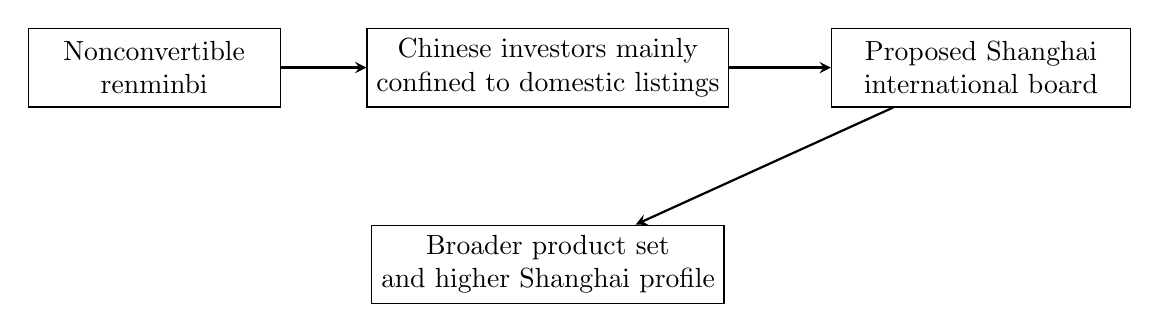
\begin{tikzpicture}[>=stealth]
\node[draw, rectangle, minimum width=3.2cm, minimum height=1cm, align=center] (rmb) at (0,0) {Nonconvertible\\renminbi};
\node[draw, rectangle, minimum width=3.5cm, minimum height=1cm, align=center] (constraint) at (5,0) {Chinese investors mainly\\confined to domestic listings};
\node[draw, rectangle, minimum width=3.8cm, minimum height=1cm, align=center] (board) at (10.5,0) {Proposed Shanghai\\international board};
\node[draw, rectangle, minimum width=3.6cm, minimum height=1cm, align=center] (products) at (5,-2.5) {Broader product set\\and higher Shanghai profile};

\draw[->, thick] (rmb) -- (constraint);
\draw[->, thick] (constraint) -- (board);
\draw[->, thick] (board) -- (products);
\end{tikzpicture}
\end{figure}

The lecture gives two motives for this board. One is to give Chinese investors access, inside China, to a wider variety of firms. The other is to raise the status of Shanghai as an international financial center. At the time of the lecture, however, the rules and timetable were still unsettled.

\subsection{Question \& Answer}

\paragraph{Question.} Is China's central market problem a lack of regulation, or a problem of clear and consistent enforcement?

\paragraph{Answer.} The lecture is very clear that the deeper problem is enforcement and application. Rules that are unclear, inconsistently applied, or weakly enforced do not create a reliable market even if the formal rulebook is extensive. The operative variable is not the number of rules, but the quality of institutional execution.

\section{How Regulators Think: Precedent, Exchange Consolidation, and Global Rulemaking}

One of the strongest moments in the lecture comes when Cha explains the difference between solving a client's problem and judging a market issue as a regulator. This is the place where the lecture most clearly moves from biography to method.

In the private sector, one is often given a client's problem and asked to help that client get where it wants to go---through an acquisition, a merger, a disposal, or some other transaction. In the public sector, by contrast, one has to ask about the effect on the market as a whole. In a compressed form, the contrast is
\begin{align}
\text{Private-side problem} &: \text{How do we help this client?} \\
\text{Regulatory problem} &: \text{What precedent does this set for the market?}
\end{align}

Cha then gives an explicit example. A group of companies requests an exemption. The request may be entirely reasonable from the point of view of that group. A lawyer would naturally fight to obtain the exemption. A regulator must ask a different sequence of questions. What precedent does this create? Is it a good precedent? If so, why should only this group receive it? Should the rule itself be amended? If not, why should the market tolerate an idiosyncratic carve-out? In schematic form,
\begin{equation}
X \Rightarrow
\begin{cases}
\text{amend the rule for all}, & \text{if } X \text{ creates a good general precedent},\\[4pt]
\text{deny the exemption}, & \text{if } X \text{ is merely client-specific or harmful}.
\end{cases}
\end{equation}

This is the lecture's clearest worked derivation, even though it is institutional rather than algebraic. We can lay it out step by step:
\begin{enumerate}
\item A firm or group asks for an exemption.
\item The reasons may be plausible from the firm's own point of view.
\item A regulator must test the request against market-wide precedent.
\item If the precedent is good, private relief is the wrong remedy; the rule should be generalized.
\item If the precedent is bad, the exemption should be denied.
\end{enumerate}

The lecture then broadens this regulator's viewpoint to the structure of exchanges themselves. Demutualization has changed what an exchange is. Once exchanges become listed corporate entities, mergers and alliances become thinkable. Cha argues that such mergers make economic sense only under specific conditions:
\begin{equation}
\text{Exchange merger viability}
\Rightarrow
(\text{product complementarity})
\land
(\text{geographic fit})
\land
(\text{political feasibility}).
\end{equation}
Even here, however, commercial logic is not enough. Exchanges retain symbolic national significance, and local politics may block what looks like a rational transaction.

A later student asks about Cha's transition from law to regulation and then to the board of HSBC. Her answer fits the same method. The major adjustment in becoming a regulator was learning not merely to improve documents but to solve public problems. That is, one stops treating the document as the object and starts treating the market consequence as the object.

The final technical question concerns Basel III. Cha does not enter into exact capital ratios, and we should not invent them here. What she does provide is a dynamic model of post-crisis regulation. After a crisis, regulation tightens; the pendulum swings too far; in calmer periods it comes back; and the next crisis tends to be different from the last. A schematic version is
\begin{equation}
C_t
\Rightarrow
\text{tighter regulation}_{t+1}
\Rightarrow
\text{overshoot}
\Rightarrow
\text{partial relaxation}
\Rightarrow
C'_{t+k}.
\end{equation}
Sarbanes-Oxley is offered as one historical example of such a response pattern after Enron. Basel III, in the lecture, plays the same role after the global financial crisis.

This leads naturally into the last issue, international harmonization. Regulators may talk for a long time about one harmonized global standard, and institutions such as the Financial Stability Board and the G20 may coordinate. But Cha's judgment is that true harmonization remains difficult because national regulators have different priorities. Coordination is possible. Complete unification is much harder.

\subsection{Question \& Answer}

\paragraph{Question.} How does a regulator's way of reasoning differ from that of a lawyer, banker, or private adviser?

\paragraph{Answer.} The regulator thinks at the level of precedent, spillover, and system integrity. The private adviser asks whether a specific client can achieve a specific objective. The regulator asks whether granting that objective in that form would distort the market, create an undesirable precedent, or require a rule change for all comparable cases. The scale of reasoning is wider.

\section{Summary}

This lecture has almost no formal mathematics in the usual sense, but it has a strong analytic spine. Cha's central claim is that markets must be understood as joint products of private intermediation and public architecture. From that starting point she moves through a sequence of concrete examples: the transformation of Hong Kong through Chinese listings, the growth of Chinese capital markets, the role of governance and enforcement, the meaning of exchange demutualization, the logic of foreign listings, and the post-crisis cycle of tighter regulation and attempted international coordination.

Shiller's closing remark captures the theme well. In a period of global expansion, somebody has to get the institutional details right. Cha's lecture is an account of what it means to do that work from inside the market itself.